\section{Numerical Discretization Error vs. Turbulence Modeling Uncertainty}\label{sec:num_vs_turb_error}

Solving continuous equations on a discrete domain creates numerical discretization error.
In RANS CFD simulations, the continuous RANS equations that define fluid flow are solved on a discrete domain known as the mesh or grid.
Numerical discretization error can be reduced by increasing the number of discrete points in the domain.
As the discretization increases and the grid spacing tends towards $0$, the numerical error approaches $0$ as well. 
This is the basis for the "Grid Convergence Study" method for quantification of numerical discretization error \cite{american_society_of_mechanical_engineers_standard_2009}.
Details of the methodology are reproduced here for clarity.

The methodology requires the use of a family of grids that are sequentially coarser but are generated using the same grid generation parameters.
This is most easily done with structured meshes where a very dense grid, which would result in minimal discretization error, is first generated.
Then each successive coarser grid level removes every other grid line in each direction.
In 2D and 3D computations, this results in the number of grid point reducing by a factor of 4 and 8 respectively, at each grid level.
It results in grids that are uniformly refined which isolates the effect of the discretization on the simulations. 

Three grids of successive refinement are required to calculate all the numerical error metrics. 
First, a representative grid size for the $i$-th grid is defined as
\begin{equation} \label{equ:grid_h}
    h_i = \left ( \frac{1}{N_i}\right )^A
\end{equation}
where $N_i$ refers to the number of degrees of freedom in the $i$th grid and $A=1/2$ for 2-D simulations and $A = 1/3$ for 3-D simulations.
SU2 uses node-centered numerics, so $N_i$ refers to the number of nodes in the grid.
The grids are ordered such that $i=1$ refers to the finest grid (most number of nodes) and $i=3$ refers to the coarsest grid.
Correspondingly, a smaller value of $h$ indicates a finer mesh with more nodes. 
Next, grid ratios are defined as 
\begin{equation}
    r_{21} = \frac{h_2}{h_1},~r_{32} = \frac{h_3}{h_2},
\end{equation}
and solution differences are defined as
\begin{equation}
    \epsilon_{21} = \phi_2 - \phi_1,~\epsilon_{32} = \phi_3 - \phi_2,
\end{equation}
where $\phi_i$ is the solution on the $i$-th grid.
Often for aerodynamics-related problems $\phi$ represents a force or moment coefficient such as $C_L$ or $C_m$.

These quantities can be used to compute the observed order of convergence, $p$, by solving the following equations using a fixed point iteration:
\begin{align}
    p & = \frac{1}{\ln{\left ( r_{21} \right )}} \left ( \ln{\left \vert \frac{\epsilon_{32}}{\epsilon_{21}} \right \vert } + q(p) \right )
    \\
    q(p) & = \ln{ \left ( \frac{r_{21}^{p} - s }{r_{32}^{p} - s}\right )}
    \\
    s & = 1\times sign \left ( \frac{\epsilon_{32}}{\epsilon_{21}}\right ).
\end{align}
The order of convergence should be close to the order of the numerical method used to solve the simulations. 
2nd order numerical methods are used for all of the RANS calculations made using SU2 and so we expect the observed order to be close to $2$.

Using the grid ratios and the apparent order of convergence, the infinite grid solution can be extrapolated as,
\begin{equation}
    \phi_{ext}^{21} = \frac{r_{21}^p\phi_1 - \phi_2}{r_{21}^p - 1}.
\end{equation}

The approximate relative fine-grid error: 
\begin{equation}
    e_a^{21} = \left \vert \frac{\phi_1 - \phi_2}{\phi_1} \right \vert,
\end{equation}
can be used to calculate the fine-grid convergence index:
\begin{equation}
    GCI_{fine}^{21} = \frac{1.25e_a^{21}}{r^p_{21}-1}.
\end{equation}
Here $1.25$ is an empirically recommended Factor of Safety based on hundreds of CFD case studies \cite{roache1998verification}.
Furthermore, the GCI can be used to express the $95\%$ confidence interval on the fine grid solution. 
The solution can be expressed as
\begin{equation} \label{equ:num_error_bars}
    \phi \approx \phi_1 \pm \left( GCI_{fine}^{21} \right)\left \vert \phi_1 \right \vert 
\end{equation}


Armed with these metrics to quantify the numerical discretization error in the CFD simulations, comparisons to the uncertainty introduced by turbulence models can be made. 
The eigenspace perturbation methodology discussed in Section \ref{sec:equips_rans_uq} only estimates uncertainties introduced by turbulence models.
The RANS CFD simulations required to quantify the uncertainties are run on grids that introduce some degree of discretization error.
The following sections explore the relationship and the relative magnitudes of the two quantities.

\subsection{NACA0012 Airfoil} \label{sec:num_err_naca0012}

The same NACA0012 case presented in Section \ref{sec:equips_naca0012} is used here. 
This case is used in the 5th and 6th Drag Prediction Workshops as a verification study \cite{levy2013summary,roy2017summary}.
The grids that were used for those verification studies are used here, details for which are shown in Table \ref{tab:naca0012_meshes}.

\begin{table}
    \renewcommand{\arraystretch}{1.2}
    \centering
    \begin{tabular}{ c|c|c|c|c } 
%  \hline
         Mesh Level & Nodes & Surface Nodes & Wall spacing & Approx. $y^+$  \\ 
         \hline
         L1 & $14,687,744$ & $4,097$ & $1.0\times10^{-7}~m$ & 0.025\\
         L2 & $3,673,856$ & $2049$ & $2.0\times10^-7~m$ & 0.05\\
         L3 & $919,424$ & $1,025$ & $4.0\times10^{-7}~m$ & 0.1\\
         L4 & $230,336$ & $513$ & $8.0\times10^{-7}~m$ & 0.2\\
         L5 & $57,824$ & $257$ & $1.6\times10^{-6}~m$ & 0.4\\
         L6 & $14,576$ & $129$ & $3.2\times10^{-6}~m$ & 0.8\\
         L7 & $3,584$ & $65$ & $6.4\times10^{-6}~m$ & 1.6\\
        
    \end{tabular}
    \caption{Details of the grid family used to perform numerical discretization error quantification for the NACA0012 case.}
    \label{tab:naca0012_meshes}
\end{table}

To be consisted with the results form the eigenspace perturbation methodology, the SST turbulence model is used for these simulations. 
The grid convergence trends for $C_L$ and $C_D$ are shown in Figure \ref{fig:naca0012_mesh_convergence}.
The $x$-axis for the figures is the representative mesh size $h$ (Equation \ref{equ:grid_h}). 
Going from right to left on the $x$-axis corresponds to increasing grid refinement, from the L7 mesh to the L1 mesh. 
As the grid refinement increases the coefficients converge towards the infinite grid solution.

Ideally, to compare the numerical discretization error and the turbulence modeling uncertainty, the finest three meshes woul

\begin{figure}
\center
\subfigure%[\label{subfig:naca0012_tmr_CL} Coefficient of pressure variation over the upper surface of the airfoil at $\alpha=10^{\circ}$]
  {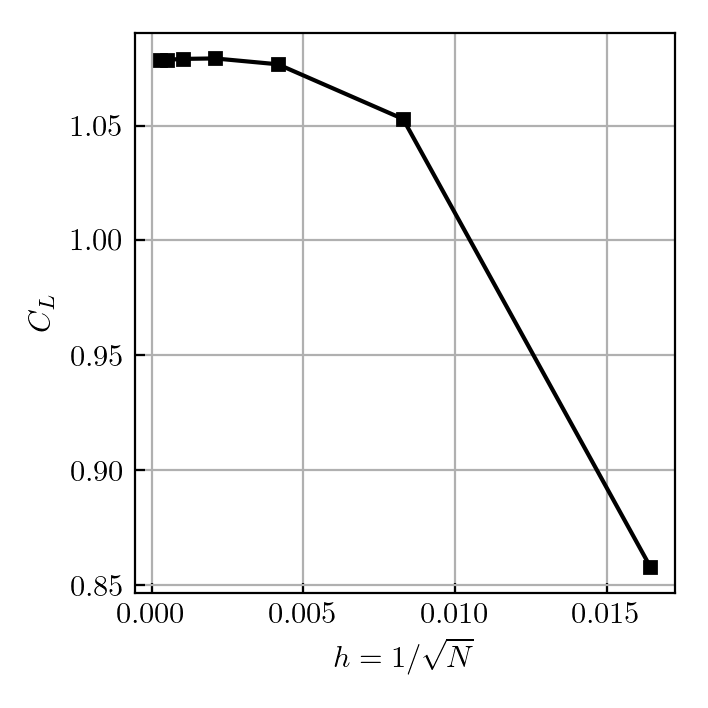
\includegraphics[width=0.48\textwidth]{code/image_gen/naca0012/images/naca0012_CL_tmr_mesh_convergence.png}}
\subfigure%[\label{subfig:naca0012_tmr_CD }Coefficient of pressure variation over the upper surface of the airfoil at $\alpha=15^{\circ}$]
  {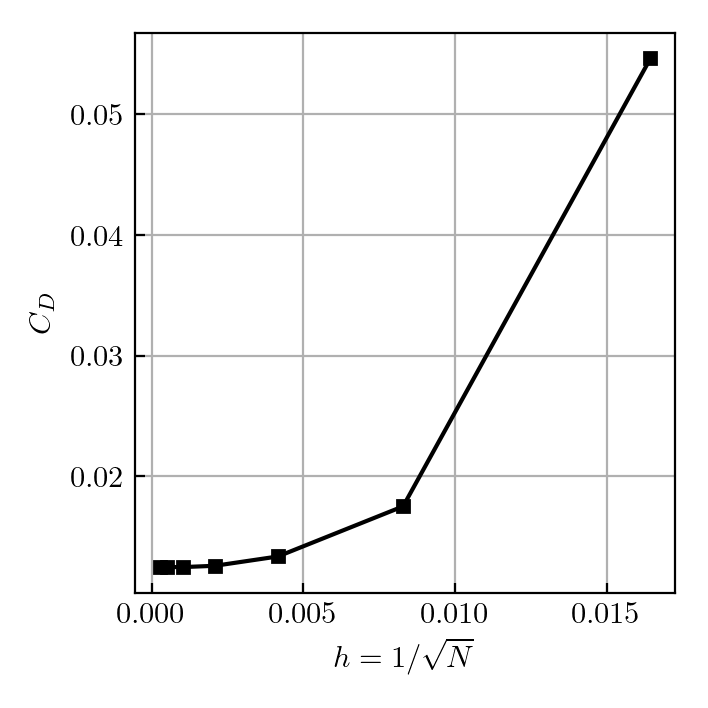
\includegraphics[width=0.48\textwidth]{code/image_gen/naca0012/images/naca0012_CD_tmr_mesh_convergence.png}}
\caption{Effects of grid refinement on $C_L$ and $C_D$ predictions at $\alpha = 10^\circ$ for the NACA0012 airfoil.}\label{fig:naca0012_mesh_convergence}
\end{figure}

For this case the $GCI_{fine}^{43} = 5.0 \times 10^{-5}$ which represents a $95\%$ confidence interval of $1$ drag count ($10^-4$). 
This is a suitably low numerical discretization error that would not adversely affect the RANS CFD simulations. 
The finer meshes, L2 and L1, are computationally expensive to perform simulations on.
So to compare the numerical discretization error and the uncertainties predicted by the eigenspace perturbation methodology, the L3, L4, and L5 meshes are used. 
The L6 mesh, which has significant numerical error as evidenced by its under-prediction of $C_L$ and over-prediction of $C_D$, is also explored to see how the RANS UQ methodology handles insufficient discretization that might not capture relevant flow features. 

